\chapter{Vlastní algoritmické řešení}
\label{ch:VlastniAlg}

V této kapitole se zaměříme na popis vlastního algoritmu pro detekci systolických vrcholů a odhad srdeční tepové frekvence z fotopletysmografických signálů.

Našim cílem je vytvořit jednoduchý a efektivní algoritmus, který poskytne spolehlivé výsledky pro různé typy PPG signálů.

\section{Předzpracování PPG signálu}
\label{sec:alg_preproc}

\subsection*{Načtení signálů}
\label{sec:alg_load}
% - Záznamy jsou uloženy v různých formátech, proto je nutné je převést do jednotného formátu.
%    - numpy řetězce, int, float, ... do jedné python knihovny.
% - Dovygenerujeme referenční TF z referenčních systolických vrcholů - použijeme stejný algoritmus pro výpočet ref TF jako pro výpočet TF z námi detekovaných vrcholů.
Jelikož pracujeme se dvěma databázemi - \emph{CapnoBase} a \emph{BUT~PPG}, výstupem po načtení signálů jsou dvě odlišné knihovny, které zpracováváme samostatně později.
Obě databáze mají odlišnou strukturu souborů a formát signálů, což vyžaduje samostatný přístup při jejich načítání.

Databáze \emph{CapnoBase} obsahuje signály uložené v \texttt{.mat} souborech.
Z každého souboru načítáme signál PPG, referenční systolické vrcholy a vzorkovací frekvenci~\cite{CapnoBase}.
Navíc si vygenerujeme referenční tepovou frekvenci (TF) z referenčních vrcholů, a to pomocí stejného algoritmu, který později použijeme pro výpočet TF z našich detekovaných vrcholů.
Pro účely čitelnější vizualizace a zpracování ukládáme též identifikátor záznamu, což jsou první čtyři znaky názvu souboru.

Oproti tomu databáze \emph{BUT~PPG} používá formát \acl{WFDB} (\acs{WFDB}) a obsahuje PPG záznamy v \texttt{.dat} a \texttt{.hea} souborech.
Tato databáze původně obsahovala 48 záznamů, které byly později rozšířeny o dalších 3~840 záznamů.
Při načítání bylo nutné zohlednit, že starší PPG signály byly uloženy v jednom kanálu, zatímco ostatní signály byly rozděleny do tří kanálů, odpovídajících třem různým barevným složkám signálu~\cite{BUT_PPG_database}.
Z novějších záznamů jsme jako referenční PPG signál vybrali pouze červenou složku, která nejvíce odpovídá standardnímu PPG signálu.

Výsledkem načtení jsou dvě knihovny, které obsahují dostupná data z~obou databází ve formátu vhodném pro další zpracování.

\subsection*{Rozdělení záznamů}
\label{sec:alg_split}
% - Dlouhé záznamy z CapnoBase můžeme rozdělit na kratší úseky, které budou zpracovány jednotlivě.
%   - Z osmiminutového záznamu vytvoříme 8x 1minutový úsek s 10ti procentním překryvem.
Záznamy v databázi \emph{CapnoBase} jsou dlouhé osm minut.
Tuto délku jsme považovali za nevhodnou pro výpočet tepové frekvence, protože výsledná hodnota TF by mohla být zkreslená kratšími úseky se zvýšenou nebo sníženou TF.
Mohlo by se tedy stát, že referenční a naše tepové frekvence by vykazovaly podobné výsledky, přestože by se v jednotlivých úsecích mohly výrazně lišit.

Proto jsme přistoupili k rozdělení každého dlouhého záznamu na kratší, minutové, segmenty, které měly desetiprocentní překryv.
Takový překryv byl zaveden proto, abychom testovali algoritmy na všech vrcholech v záznamu.
Výsledné minutové úseky byly dále považovány za samostatné signály, které byly zpracovány jednotlivě.

\subsection*{Filtrace}
\label{sec:alg_filter}
% - Bandpass filter - Butterworthův filtr - vlastní nastavení.
% - Na konec signál standardizujeme od -1 do 1.
Po načtení a případném rozdělení záznamů následovalo filtrování signálu, které je klíčové pro odstranění šumu.
Pro tento účel jsme aplikovali pásmový filtr typu Butterworth, jehož parametry jsme nastavili s ohledem na fyziologické vlastnosti PPG signálu.

Konkrétně jsme použili pásmový filtr druhého řádu s dolní mezní frekvencí 0,5~Hz (30 úderů za minutu) a horní mezní frekvencí 3,35~Hz (201 úderů za minutu).
Tento rozsah byl zvolen tak, aby odstranil velmi pomalé změny v signálu, například dechovou frekvenci, a zároveň potlačil vysokofrekvenční šum, který by mohl negativně ovlivnit detekci vrcholů.
% order explain
% normované mezní frekvence vzhledem k Nyquistově frekvenci - explain
% aplikace nulofázového filtru - explain

Po filtraci jsme signál standardizovali do rozsahu od \(-1\) do \(1\).
Tato normalizace zajišťuje jednotné měřítko napříč všemi záznamy, což je důležité pro následné kroky detekce, kde algoritmus pracuje s relativními prahy a hodnotami.

Výsledkem těchto kroků byl očištěný a normalizovaný signál, připravený pro detekci systolických vrcholů.
Na obrázku~\ref{fig:filter-peaks} jsou ilustrovány různé části původních a filtrovaných signálů (oba signály jsou pro lepší přehlednost standardizovány).

\section{Detekce vrcholů}
\label{sec:alg_peaks}
% - Detekce vrcholů v 5ti sekundových oknech, které se z 50ti procent překrývají.
%   - koukáme na 5 sekund, pak posuneme o 2,5 sekundy a znovu koukáme na dalších 5 sekund.
% - standardizace signálu v okně: -1 do 1
% - nastavení prahů - min_peak_height (lokální brute force 0,3), min_peak_distance (200 bps)
% - lokal max detektor:
%       - koukne na každý vzorek a porovná ho s předchozím a následujícím vzorkem.
%       - pokud je větší než oba AND je větší než nastavené prahy, tak je to vrchol.
% - na konci jen odstraníme vrcholy, které jsou na stejném vzorku (kvůli překrývání oken), protože chceme v budoucnu pracovat i s tím, kolik jsme našli vrcholů v okně - duplikáty by nám to zkreslily.

\section{Výpočet tepové frekvence}
\label{sec:alg_hr}
% - výpočet IBI z detekovaných vrcholů + popsat matematicky IBI
% - výpočet TF z IBI: TF = 60 / median(IBI) OR TF = 60 / mean(IBI) -- my použijeme median protože počítáme, že se v minutovém úseku (nebo desetisekundovém úseku BUT PPG) může objevit nějaký výrazný artefakt, který by nám zkreslil výpočet průměru. Pro delší úseky bychom použili průměr.
% - stejný postup je i pro výpočet ref TF z referenčních vrcholů (viz. \ref{sec:alg_load}) = můžeme porovnat s naším výstupem.
%%%%%%%%%%%%%%%%%%%%%%%%%%%%%%%%%%%%%%%%%%%%%%%%%%%%%%%%%%%%%%%%%%%%%%%%%%%%%%%%%%%%%
%%%%%%%%%%%%%%%%%%%%%%%%%%%%%%%%%%%%%%%%%%%%%%%%%%%%%%%%%%%%%%%%%%%%%%%%%%%%%%%%%%%%%
% Po detekci systolických vrcholů jsme mohli přistoupit k výpočtu tepové frekvence.

% Základní veličinou pro tento výpočet je interval mezi dvěma po sobě následujícími vrcholy, označovaný jako inter-beat interval (IBI).
% Matematicky lze tento interval vyjádřit jako \(\mathrm{IBI}_i = t_{i} - t_{i-1}\), kde \(t_i\) je čas detekce \(i\)-tého vrcholu.
% Hodnoty \(\mathrm{IBI}\) jsou vyjádřeny v sekundách.

% Z každé série detekovaných vrcholů jsme získali množinu \(\mathrm{IBI}\), ze které jsme následně odvodili tepovou frekvenci.
% Výpočet TF probíhal podle vztahu:
% \[
% \mathrm{TF} = \frac{60}{\mathrm{median}(\mathrm{IBI})},
% \]
% kde \(\mathrm{median}(\mathrm{IBI})\) označuje medián všech intervalů v daném úseku.
% Použití mediánu bylo zvoleno záměrně, protože u kratších segmentů (například minutových úseků u CapnoBase nebo desetisekundových u BUT~PPG) se může objevit výrazný artefakt, který by zkreslil aritmetický průměr.
% Pro delší úseky bychom naopak preferovali průměr, protože je citlivější na menší změny v rytmu.

% Stejným postupem jsme počítali také referenční tepovou frekvenci, a to přímo z referenčních vrcholů dostupných v databázi (viz \autoref{sec:alg_load}).
% Tento přístup nám umožňuje přímo porovnat naše výsledky s referenčními hodnotami a vyhodnotit tak přesnost navrženého algoritmu.

\begin{figure}[t]
	\centering
	\vspace{-10mm}
	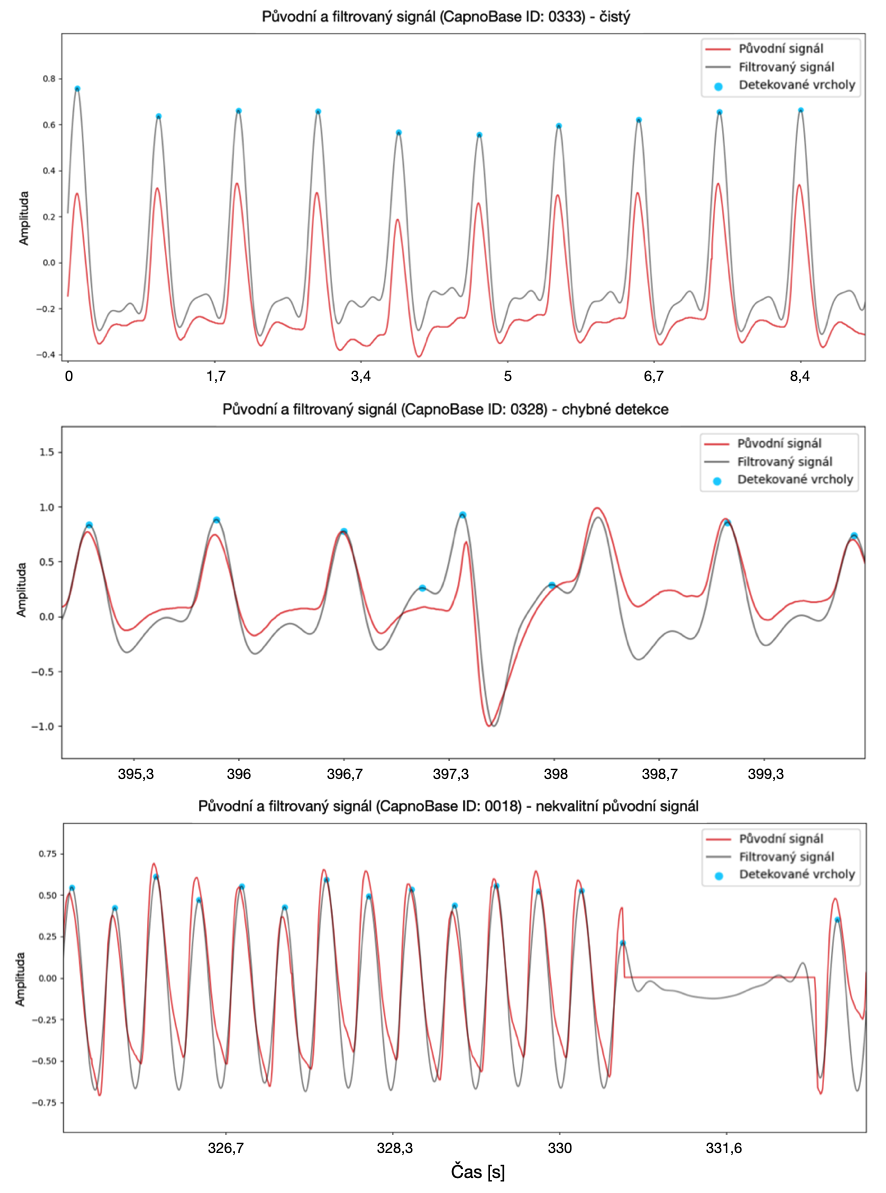
\includegraphics[width=1\textwidth]{./obrazky/MyFilterPeaks.png}
	\caption[Vlastní zpracování signálů]{...}
	\vspace{-15mm}
	\label{fig:filter-peaks}
\end{figure}